\section{Essential code snippets behind the system}
The main part of this project is to develop a client-server communication system, with the purpose of producing a physical simulation on how a centralized system can contribute to an improved traffic flow. Due to the nature of this project, no graphical user interfaces has been developed. Hence, it is deemed necessary to present key parts of the code that are responsible for such a system to work. This section will therefore elaborate, in detail, how essential code snippets are interacting with each to produce the result.

Furthermore, the code that has been written during this project has been written in the languages Python and C\# using Pycharm and Rider IDE respectively. Therefore, syntax highlighting has also been used to best simulate the same syntax highlighting used in both IDE respectively. In addition, some artistic freedom has been used to present the code snippets; the symbol \verb|...| has been used to indicate irrelevant code to the current discussion and the symbol  \textcolor{red}{$\hookrightarrow$} simply means that the line of code following \textcolor{red}{$\hookrightarrow$} is on the same line above but is broken up due to lack of space. Also, each code snippets starts with the class and method it belongs to.
\subsection{Initialization}\label{initialization}
\subsubsection{Client.py}
The client package is an essential module in the Raspberry Pi vehicles for the success of this project. The client class is mainly responsible for connecting, handling, and sending data to the server. The client class does not aim to be used alone but rather as a superclass for other IoT devices. Hence, it should be inherited and handle everything that pertains to client-server communication in the background.

The client's init method does several things: It reads from the config.json file to store the defined host and port it will use to establish a connection to the server.
\begin{python}
class Client:
	def __init__(self, properties=None, **kwargs):
		...
		with open("client/config.json") as f:
			config = json.load(f).get('client')
			if config is not None:
				self.__uri = f"://{config.get('host')}:{config.get('port')}/{self.__class__.__name__.lower()}sHub"
				self.__delay = config.get('delay')
		...
\end{python}

Then, it starts a negotiation process with the server, where it receives a connection id that the client will use during its connection lifetime to the hub.

\begin{python}
class Client:
	def __init__(self, properties=None, **kwargs):
		...
		urllib3.disable_warnings()
		response = requests.post(f"http{self.__uri}/negotiate?negotiateVersion=0", verify=False)
		self.connection_id = response.json().get("connectionId")
		self.websocket_uri = f"ws{self.__uri}?id={self.connection_id}"
		...
\end{python}

The client also gives itself a random id stored as one of its properties. The client's id is also stored on the server and is mainly used to retrieve and update the client's information.

Furthermore, \verb|Client.__init__| also stores a dictionary of events.
\begin{python}
class Client:
	def __init__(self, properties=None, **kwargs):
		...
		self.subscribed_events = {
			"disconnect": self.disconnect,
			"force_patch": self.force_patch,
			"continuously_patch": self.continuously_force_patch
		}
		...
\end{python}

Values in this dictionary are references to functions in this class and is used to invoke certain behaviours by the server. For instance, \newline\verb|await Clients.Client(Context.ConnectionId).SendAsync("disconnect");| from the server will call \verb|def disconnect(self)| in the client. 

\subsubsection{Vehicle.py}
The vehicle class contains all the data and methods of the vehicle. Furthermore, \verb|class Vehicle(Client)| inherits the client class which enables \verb|Vehicle| to perform all the necessary operations to establish connection upon initiation. An important remark is that \verb|Client| performs the negotiation to the server using endpoint \newline \verb|{self.__class__.__name__.lower()}sHub/negotiate?negotiateVersion=0| meaning that through inheritence and initialization of \verb|Vehicle|, the subclass negotiates with the endpoint  \verb|vehiclesHub/negotiate?negotiateVersion=0|, which is mapped in \verb|Program.cs| with
\begin{csharp}
...
app.MapHub<VehiclesHub>("/vehiclesHub");
...
\end{csharp}

Furthermore, \verb|Vehicle| also reads from \verb|config.json| to define it's initial properties with the snippet shown below:
\begin{python}
class Vehicle(Client):
	def __init__(self, properties=None, **kwargs):
		...
		if properties is None and len(kwargs) == 0:
			with open("client/config.json") as f:
				config = json.load(f).get('vehicle')
				if config is not None:
					self.properties.update(config)
		...
\end{python}

\verb|Vehicle| also utilizes the property builder of \verb|Client|.

\begin{python}
class Vehicle(Client):
	def __init__(self, properties=None, **kwargs):
		...
		self.property_builder(
			required={'length', 'height', 'width', 'mass'},
			optional={'velocity': 0, 'position': 0, 'travel_plan': None},
		)
		...
\end{python}

In short, the property builder is used to define the required properties of the vehicle class. The meaning is to restrict somewhat what data the vehicle class should contain. If one should directly initialize Vehicle without using config.json, one must assign values to length, height, width, and mass.

Lastly, \verb|Vehicle| adds subscribed events that the server can invoke:
\begin{python}
class Vehicle(Client):
	def __init__(self, properties=None, **kwargs):
		...
		self.subscribed_events.update({
			"adjust_velocity": self.adjust_velocity
		})
\end{python}

Likewise, as in \verb|Client|, should other events be required for a vehicle, one can add it to the dictionary as proposed above.
\subsection{Handshake and listener}\label{handshake}
After initializing the vehicle class as a client with
\begin{python}
async def main():
	...
	client = Vehicle()
	...
\end{python}
then the client's \verb|listen| method can be called:
\begin{python}
async def main():
	...
	listener = asyncio.create_task(client.listen())
	...
\end{python}
The listener method is responsible for handling responses and requests from the server. Hence, it must run concurrently as the vehicle continuously sends data to the server.

When the listener is called, the client performs the following code:
\begin{python}
class Client:
...
	async def listen(self):
	async with websockets.connect(self.websocket_uri) as websocket:
		self.__websocket = websocket
		await self.__handshake()
		await self.__listen()
...
\end{python}
The method first opens a WebSocket connection using the stored URI and stores this as a private variable. Then, a handshake with the server is performed:
\begin{python}
class Client:
...
	async def __handshake(self, protocol: str = "json", version: int = 1):
		data = self.signalr_encode_message({"protocol": protocol, "version": version})
		await self.__websocket.send(data)
		response = self.signalr_decode_message(await self.__websocket.recv())
		if "error" in response:
			print(response)
		else:
			await self.send_non_blocking("AddClient", self.properties)
...
\end{python}

The code above describes the handshake process between the client and the server. First, the client informs the server of the protocols it will use throughout its lifetime. Then, it stores the client, in this case, the vehicle, to the server using the defined properties.

Further elaboration, the client invokes the method
\begin{csharp}
public partial class VehiclesHub : Hub
{
	...
	public async Task AddClient(JsonDocument jsonDocument) {...}
	...
}
\end{csharp}
on the server. This method first creates a vehicle with all the provided information sent by the client
\begin{csharp}
public partial class VehiclesHub : Hub
{
	...
	public async Task AddClient(JsonDocument jsonDocument)
	{
		...
		var vehicle = Vehicle.Create(jsonDocument);
		...
	}
	...
}
\end{csharp}
using the static method defined by the Vehicle model. In addition, it assigns the travel plan to the vehicle by using values defined by config.json from the client:
\begin{json}
{
	...
	"vehicle": {
		...
		"travel_plan": {
			"start": {
				"road": 0,
				"lane_reversed": false
			},
			"end": {
				"road": 0,
				"lane_reversed": false
			}
		}
	}
}
\end{json}

Furthermore, the vehicle's current lane is also assigned to track which lane the vehicle is driving on. Then, \verb|public class VehiclesHubDatabase| adds the \verb|Vehicle|, together with its connection id \verb|Context.ConnectionId| for easy retrieval.

Moreover, for the sake of the demo, the server is also instructed to wait for a second vehicle to connect before allowing the vehicles to drive
\begin{csharp}
public partial class VehiclesHub : Hub
{
	...
	public async Task AddClient(JsonDocument jsonDocument)
	{
		...
		vehicle.Velocity = 0;
		_database.Update(vehicle);
		await Clients.Client(Context.ConnectionId).SendAsync("adjust_velocity", vehicle);
		await WaitForVehicles(vehicle, _database.SpeedLimit, 2);
	}
	...
}
\end{csharp}
by first setting the vehicle's velocity to zero, updating the new velocity in the database, and adjusting the velocity of the client to zero. Lastly, it calls the \verb|WaitForVehicles| method, which will adjust every client's velocity to the defined \verb|SpeedLimit| in \verb|VehiclesHubDatabase|.

\subsection{Patch}
After initialization and handshake elaborated in \hyperref[initialization]{\ref{initialization} Initialization} and \hyperref[handshake]{\ref{handshake} Handshake and listener} respectively, the Raspberry Pi vehicles starts to drive into an intersection simultaneously. Throughout the journey the cars are continuously patching to the server, by calling the client's \verb|async def send\_patch| method.

\begin{python}
class Client:
	...
	async def send_patch(self, **kwargs) -> None:
		if self.properties_has_changed(**kwargs) or self.__continuously_patch:
			await self.send_invocation("patch", self.properties)
		else:
			await asyncio.sleep(self.__delay)
\end{python}

As seen above \pythoninline{send\_patch} calls the \pythoninline{async def send_invocation} method, which communicates the vehicle's current information by invoking \newline
\verb|public async Task Patch| on \verb|VehiclesHub|.

The patch method on \verb|VehiclesHub| is responsible for handling the behaviour, specifically adjusting the velocity of individual vehicles:
\begin{csharp}
public partial class VehiclesHub : Hub
{
	...
	public async Task Patch(JsonDocument jsonDocument)
	{
		var vehicle = Vehicle.Create(jsonDocument);
		_database.Update(vehicle);
		vehicle = _database.Fetch(vehicle);
		...
	}
}
\end{csharp}
The snippet above shows that the method first creates a new vehicle using the information provided by the \verb|Client|. However, since this new vehicle does not contain all the information, such as the travel plan, the method first update the existing vehicle in the database in order to refresh the vehicle with the available information. It then fetch the same vehicle that was stored in the handshake, mentioned in \hyperref[handshake]{\ref{handshake} Handshake and listener}. Assuming that the vehicle has been successfully retrieved it will then handle this vehicle accordingly:
\begin{csharp}
public partial class VehiclesHub : Hub
{
	...
	public async Task Patch(JsonDocument jsonDocument)
	{
		...
		await HandleIntersection(vehicle);
		await HandleInsideIntersection(vehicle);
		await HandleEndOfRoute(vehicle);
		...
	}
}
\end{csharp}
Shortly summarized \verb|HandleIntersection| is responsible to adjust the velocity of every vehicle approaching the intersection to avoid collisions. Furthermore, \verb|HandleInsideIntersection| increases the speed to \verb|VehiclesHubDatabase| defined \verb|SpeedLimit|. Lastly, \verb|HandleEndOfRoute| ensure that any vehicles that has completed their journey, defined during the handshake, terminates their connection with the server.
\subsection{VehiclesHubDatabase}
The \verb|VehiclesHubDatabase| played a key role in this project. Coming to the realization on \hyperref[phase3]{\ref{phase3} Phase 3 - Signal R} the project needed a database that could handle the continuous changes in each \verb|Vehicle| position in real time. During research the group was unable to conclude on any databases that would fit our requirement. Hence, \verb|VehiclesHubDatanbase| was created to serve as a live in-memory database that could continuously update the positions of each vehicle on each lane.
\begin{figure}[h!]
	\centering
	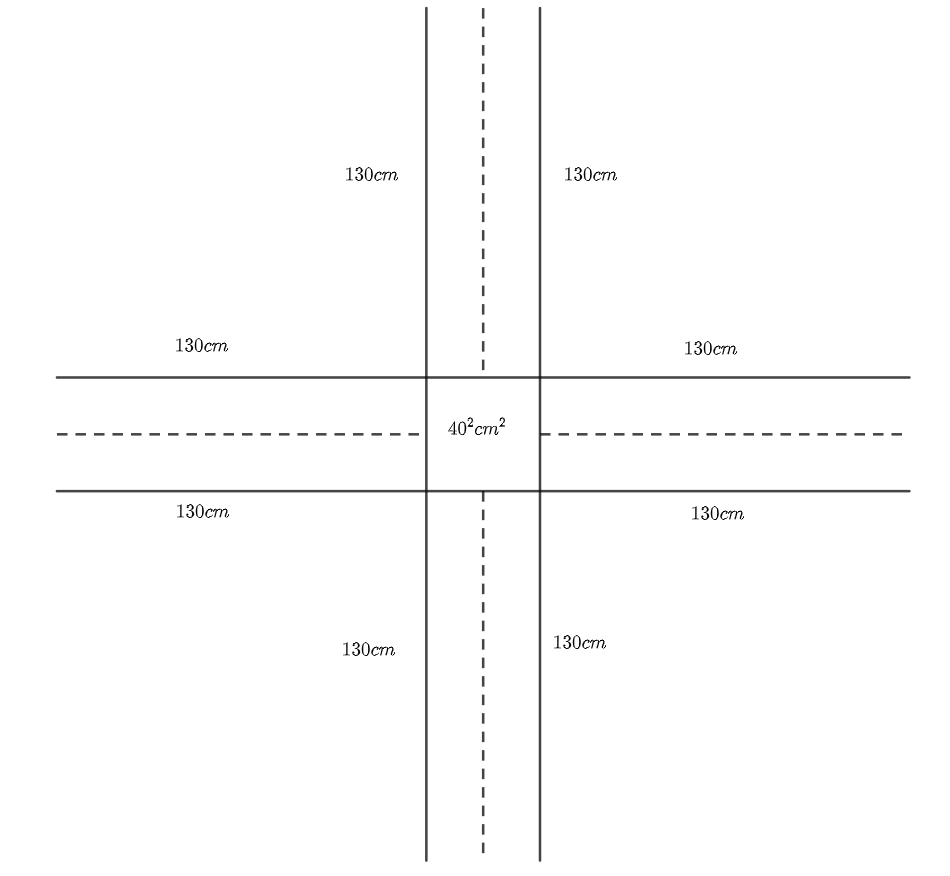
\includegraphics[width=1\linewidth]{figures/intersection_concept}
	\caption{This figure shows two roads each with two lanes and a total length of 300cm. The overlapping part forms a square which is the intersection. This configuration was heavily considered when creating representational models on the server, and also used for the demo as a result.}
	\label{fig:intersectionconcept}
\end{figure}

Before starting with \verb|VehiclesHubDatabase|, it was required to define what a road, lane and intersection is, respectively. Thus, \verb|Road.cs|, \verb|Lane.cs| and \verb|Intersection.cs| was developed. Consequently, \verb|VehiclesHubDatabase| was created.
\begin{csharp}
public class VehiclesHubDatabase : IVehiclesHubDatabase
{
	private readonly Intersection _intersection;
	
	private readonly HashSet<Vehicle> _vehicles = new();
	private readonly HashSet<Lane> _lanes = new();
	public int Count => _vehicles.Count;
	private readonly Dictionary<string, Vehicle> _connectionIds = new();
	private readonly Dictionary<Vehicle, string> _vehiclesConnectionId = new();
	...
	public double SpeedLimit => 80;
	...
}
\end{csharp}

Currently, \verb|VehiclesHubDatabase| only holds one intersection, due to time constraint this was not extended for a configuration with multiple intersections. Moreover, both vehicles and lanes are stored inside a hashset for fast retrieval. In addition, \verb|Count| is used in \verb|WaitForVehicles|, elaborated in sub-section \hyperref[handshake]{\ref{handshake} Handshake and listener}, and \verb|_connectionId| and \verb|_vehiclesConnectionId| is used during \verb|Patch| to invoke \verb|adjust_velocity| on individual vehicles. While, \verb|SpeedLimit| defines the upper speed vehicles are limited to on the two roads shown in \hyperref[fig:intersectionconcept]{Figure \ref{fig:intersectionconcept}}.

The road configuration found in \hyperref[fig:intersectionconcept]{Figure \ref{fig:intersectionconcept}} is defined in the constructor using a builder pattern.
\begin{csharp}
public class VehiclesHubDatabase : IVehiclesHubDatabase
{
	...
	public VehiclesHubDatabase()
	{
		_intersection = new Intersection().
			AddRoad(new Road {Length = 300}.
				AddLane(null, true).
				AddLane()).
		AddRoad(new Road {Length = 300}.
				AddLane(null, true).
				AddLane());
		
		_intersection.ConnectedLanes().
			ForEach(lane => _lanes.Add(lane));
	}
	...
}
\end{csharp}

Lastly, \verb|VehiclesHubDatabase| is added as a singleton service in \verb|Program.cs| to ensure that we have a static database throughout the lifetime of the program:
\begin{csharp}
...
builder.Services.AddSingleton<IVehiclesHubDatabase>(new VehiclesHubDatabase());
...
\end{csharp}

It is also worth to mention some of the core  functionalities of \verb|VehiclesHubDatabase|:

\subsubsection{Adding vehicles}
Calling the \verb|Add| method makes it possible to add vehicles:
\begin{csharp}
public class VehiclesHubDatabase : IVehiclesHubDatabase
{
	...
	public void Add(Vehicle vehicle, string? connectionId = null) {...}
	
	public void Add(Vehicle vehicle, Lane? lane = null) {...}
	...
}
\end{csharp}

\subsubsection{Removing vehicles}
Removing vehicles can be achieved by calling the \verb|Remove| method:
\begin{csharp}
public class VehiclesHubDatabase : IVehiclesHubDatabase
{
	...
	public void Remove(Vehicle vehicle) {...}
	...
}
\end{csharp}

\subsubsection{Updating vehicles}
Updating either a specific information of a vehicle or all vehicles can be done by calling the \verb|Update| method:
\begin{csharp}
public class VehiclesHubDatabase : IVehiclesHubDatabase
{
	...
	public void Update(Vehicle? vehicle = null) {...}
	...
}
\end{csharp}

\subsubsection{Fetching vehicles}
One can fetch an existing vehicle from the database by passing a vehicle with the same GUID with:
\begin{csharp}
public class VehiclesHubDatabase : IVehiclesHubDatabase
{
	...
	public Vehicle? Fetch(Vehicle vehicle) {...}
	...
}
\end{csharp}

\subsubsection{Get the connection Id of a particular vehicle}
By passing a vehicle into
\begin{csharp}
public class VehiclesHubDatabase : IVehiclesHubDatabase
{
	...
	public string? ConnectionId(Vehicle vehicle) {...}
	...
}
\end{csharp}
one can retrieve the connection Id that the given vehicle is using.

\subsubsection{Find vehicles approaching the intersection}
Maybe the most important feature of \verb|VehiclesHubDatabase| is the two method shown below:
\begin{csharp}
public class VehiclesHubDatabase : IVehiclesHubDatabase
{
	...
	public IEnumerable<Vehicle> NextVehiclesIn() {...}
	public IEnumerable<Vehicle> OnlyFirstIntoNextVehiclesIn() {...}
}
\end{csharp}
The first method \verb|NextVehiclesIn| returns a list of vehicles currently approaching the intersection defined in the constructor, ordered with respect to the vehicle closest to the intersection. The latter method \verb|OnlyFirstIntoNextVehiclesIn| returns an ordered list of the closest vehicle per lane.
\subsection{RoutePlanner and SetTravelPlan}
\verb|RoutePlanner|  is a class that determines and keep track of the \verb|Vehicle|'s journey. \verb|RoutePlanner| saves segments of lanes and intersections as nodes in a linked list:
\begin{csharp}
public class RoutePlanner
{
	private LinkedList<IRoadComponent> _visitedNodes = new();
	private LinkedList<IRoadComponent> _travelPlan = new();
	...
}
\end{csharp}
The variable \verb|_travelPlan| stores all the nodes that \verb|Vehicle| will traverse through in succession. Whenever \verb|Vehicle| has traversed the whole length of a node, the node moves to the tail of \verb|_visitedNodes|. Thus, it provides an easy way to keep track of the \verb|Vehicle|'s whereabouts.

During the handshake, described in \secref{handshake}, \verb|Vehicle| builds the \verb|_travelPlan| through its \verb|SetTravelPlan| method:
\begin{csharp}
public class Vehicle : IDevice
{
	...
	public void SetTravelPlan(Lane startLane, Lane? endLane = null)
	{
		var reversed = startLane.Reversed;
		var startNode = startLane.Node();
		var intersections = 
			reversed ? 
				startLane.CurrentRoad()?.Intersections.OrderByDescending(kvp => kvp.Key) : 
				startLane.CurrentRoad()?.Intersections.OrderBy(kvp => kvp.Key);
		...
	}
	...
}
\end{csharp}
By taking in the \verb*|startLane| and \verb*|endLane|, representing where \verb*|Vehicle| should start and end its journey, it first segments the \verb*|startLane| into a \verb*|LaneNode| and then find all the intersections on this current \verb*|Lane|, and order them chronologically depending of the lane is \verb*|Reversed| or not. \verb|SetTravelPlan| will further on iterate through all the \verb*|Intersections| and append a \verb|LaneNode| and an \verb|IntersectionNode| to \verb|RoutePlanner| for each \verb*|Intersection|.
\begin{csharp}
public class Vehicle : IDevice
{
	...
	public void SetTravelPlan(Lane startLane, Lane? endLane = null)
	{
		...
		var prevPos = reversed ? startLane.Length : 0.0;
		Intersection? intersectionConnectedToEndLane = null;
		
		if (intersections != null)
			foreach (var (position, intersection) in intersections)
			{
				startNode.Length = Math.Abs((int) (prevPos - position - (reversed ? intersection.Length : 0)));
				_route.AddComponent(startNode).AddComponent(intersection.Node());
				prevPos = position + (reversed ? 0 : intersection.Length);
				if (endLane == null) continue;
				if (!intersection.ConnectedRoads.ContainsKey(endLane.CurrentRoad() ?? new Road())) continue;
				intersectionConnectedToEndLane = intersection;
				break;
			}
		...
	}
	...
}
\end{csharp}
The above loop will iterate until one of the \verb*|Intersection| is connected to the \verb*|endLane| or until all the \verb*|Intersection|s are exhausted. In the end, \verb*|SetTravelPlan| will append the last segment of \verb*|startLane| or the remaining segment of \verb*|endLane| should \verb*|endLane| either be defined, and connected to one of \verb*|startLane|s intersections, or is equal to \verb*|startLane|.

The main reason for creating \verb*|RoutePlanner| in this project was mainly to answer the following questions:
\begin{itemize}
	\item Is \verb*|Vehicle| currently inside an intersection?
	\item Is \verb*|Vehicle| currently on a lane?
	\item Which intersection is the next intersection for this \verb*|Vehicle|?
	\item How far is \verb*|Vehicle| away from the next intersection?
\end{itemize}
By using \verb*|RoutePlanner|, we were able to answer the questions above with the following implementations respectively:
\begin{csharp}
public class Vehicle : IDevice
{
	...
	public bool InIntersection() => 
		_route.CurrentNode()?.Value is IntersectionNode;
	public bool OnRoad() => 
		_route.CurrentNode()?.Value is RoadNode or LaneNode;
	public IntersectionNode? NextIntersection() =>
		OnRoad() ? _route.NextNode()?.Value as IntersectionNode : null;
	public double ToNextIntersection()
	{
		if (InIntersection())
			return 0;
		if (OnRoad() && NextIntersection() != null)
			return Math.Abs(Position - _route.DistanceWithCurrentNode);
		return -1;
	}
	...
}
\end{csharp}

